\begin{figure}[!htbp]
  \centering
  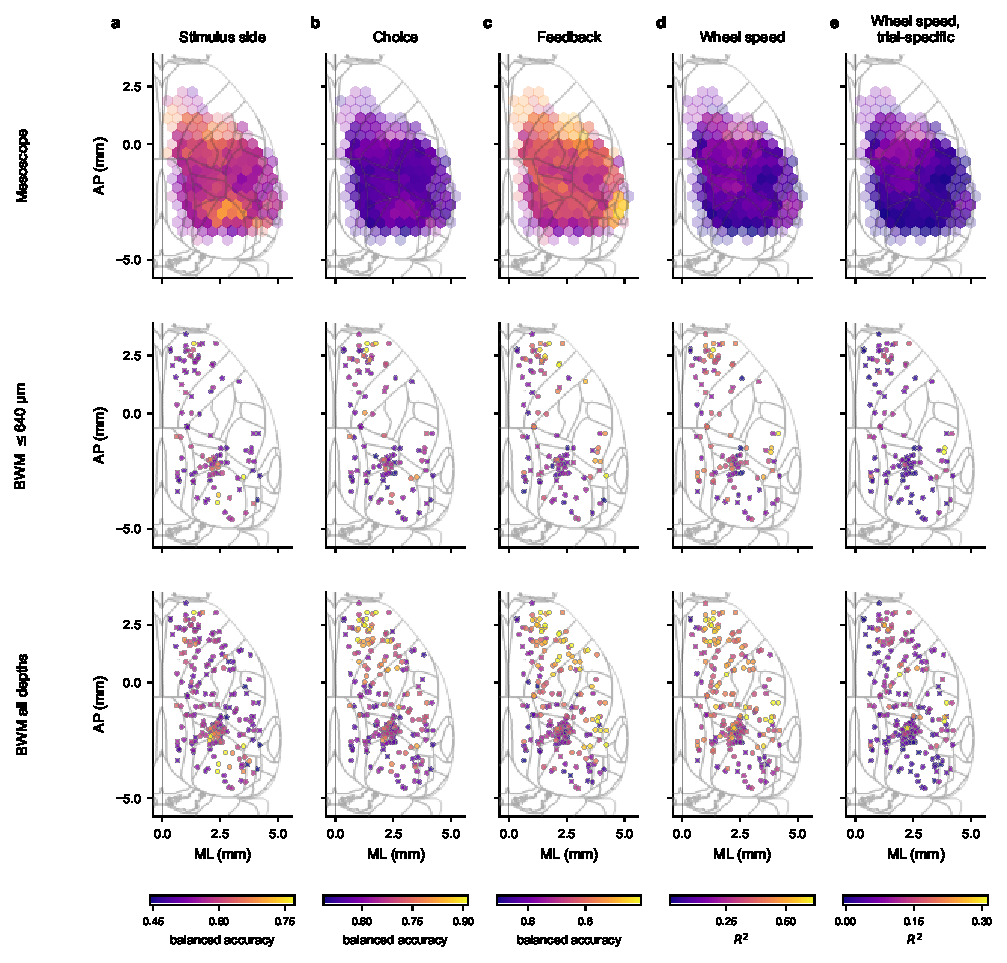
\includegraphics[width=\linewidth,height=0.8\textheight,keepaspectratio]{figures/decoding_top10.pdf}
  \caption{\textbf{Decoding from the best 10 neurons}. Top row: mesoscope decoding from the 10 highest-ranked neurons in each session and 0.5\,mm hexagon (vertex to vertex), averaged over sessions. Opacity represents the number of animals (full at $\geq$4). Middle and bottom rows: BWM decoders fit to the 10 highest-ranked neurons on each probe, using units within 640\,$\mu$m of the pia by Allen CCF streamline depth and at all depths, respectively. Each semi-transparent dot is at the probe's Alyx trajectory entry point. Hemispheres are folded onto the right. Sessions require at least 50 trials and bins or probes need at least 20 neurons. Decoding scores are available for 149 mesoscope sessions, 108 superficial BWM insertions and 207 all-depth BWM insertions. Each variable has a colour scale shared across rows, spanning the 1st to 99th percentiles of its plotted scores. Ranking was repeated on the training trials of each outer fold. Binary variables use $|\mathrm{AUC}-0.5|$. Both wheel targets use the highest signed Pearson $r$ with raw wheel speed across all wheel bins. Wheel scores require ten defined correlations per training fold. \textbf{a} Stimulus side, balanced accuracy (chance 0.5). \textbf{b} Choice. \textbf{c} Feedback. \textbf{d} Wheel speed, cross-validated $R^2$. \textbf{e} Trial-specific wheel speed, $R^2$.}
  \label{fig:decoding_top10}
\end{figure}
